\documentclass{article}
\usepackage[utf8]{inputenc}
\usepackage{amssymb}
\usepackage{amsmath}
\usepackage{float}
\usepackage{epstopdf}
\usepackage{moreverb}
\usepackage{multicol}
\usepackage{listings}
\usepackage{mathrsfs}
\usepackage{graphicx}
\usepackage{cite}
\usepackage{tabularx}
\usepackage{listings}
\usepackage{subcaption}
\newcommand{\R}{\mathbb{R}}
\newcommand{\overbar}[1]{\mkern 1.5mu\overline{\mkern-1.5mu#1\mkern-1.5mu}\mkern 1.5mu}
\newcommand{\pdiff}[2]{\frac{\partial {#1}}{\partial {#2}}}


\bibliographystyle{plain}
\title{APPM 5720 Homework 5}
\author{Wil Boshell, Fortino Garcia, Alex Rybchuk, Parth Thakkar}
\date{March 08, 2018}


\begin{document}

\maketitle

\maketitle

\section{Mapping with Straight-Sided Quadrilaterals}
In order to move from one-dimensional DG methods to two-dimensional DG methods, a mapping between the domain of the geometry and the reference domain $[-1,1]^2$ is required. One way to achieve this is with a simple bilinear mapping,

\begin{equation}
X(r,s) = \alpha_1 + \alpha_2r + \alpha_3s + \alpha_4rs, \\
Y(r,s) = \beta_1 + \beta_2r + \beta_3s + \beta_4rs
\end{equation} 

\noindent The value of the coefficients $\alpha_i$, $\beta_i$ can be found by evaluating $X(r,s)$ in each of the corners of the reference domain

\begin{equation}
    \begin{bmatrix}
      x_1 \\
      x_2 \\
      x_3 \\
      x_4 
    \end{bmatrix}
    =     
    \begin{bmatrix}
      1 & -1 & -1 & 1 \\
      1 & 1 & -1 & -1 \\
      1 & 1 & 1 & 1 \\
      1 & -1 & 1 & -1
    \end{bmatrix}
    \begin{bmatrix}
      \alpha_1 \\
      \alpha_2 \\
      \alpha_3 \\
      \alpha_4 
    \end{bmatrix}.
\end{equation}

\noindent This mapping is demonstrated below.

\begin{figure}[H]
  \centering
  \begin{minipage}{.4\textwidth}
    \centering
  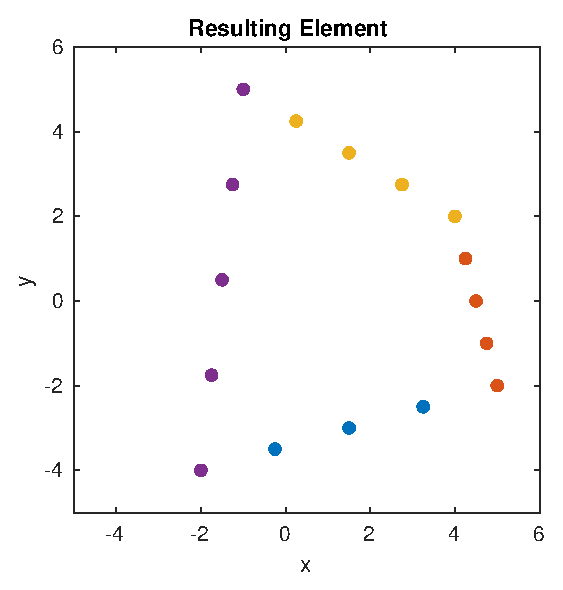
\includegraphics[width=\linewidth]{media/5-1-xy.eps}
  \end{minipage}%
  \begin{minipage}{.4\textwidth}
    \centering
  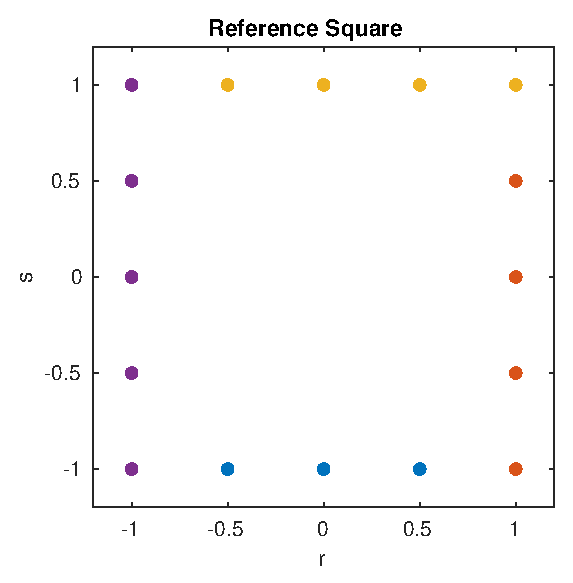
\includegraphics[width=\linewidth]{media/5-1-rs.eps}
  \end{minipage}%
  \caption{Mapping from the element domain to the reference domain $[-1,1]^2$.}
\end{figure}

\noindent With this mapping, integrals of functions in the $(x,y)$ domain can be computed through a change of variables

\begin{equation}
\int \int f(x,y) dx dy = \int \int f(x(r,s), y(r,s)) |J| dr ds,
\end{equation} 

\noindent where

\begin{equation*}
|J| =    \lvert \begin{bmatrix}
      \frac{dx}{dr} & \frac{dx}{ds}\\
      \frac{dy}{dr} & \frac{dy}{ds}
    \end{bmatrix} \rvert
\end{equation*}

In order to verify this mapping, the area of a perturbed grid with straight-sided edges was calculated. 

The value of area was found to be independent of the grid resolution as well as the degree of quadrature. This behavior is expected because here the element domain maps exactly to the reference domain.

% \begin{figure}[H]
%   \centering
%   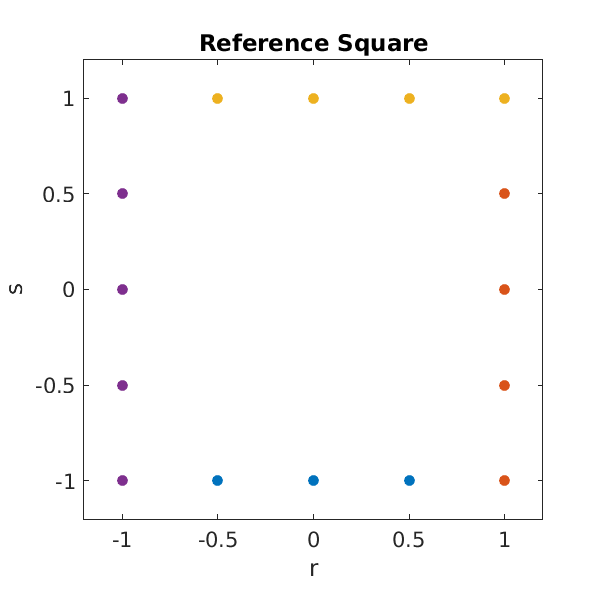
\includegraphics[width=\linewidth]{media/5-1-rs.png}
  
%   \caption{Mapping from the element domain to the reference domain $[-1,1]^2$.}
%   \label{fig:spatDer}
% \end{figure}

A similar area calculation was carried out for elements with curvilinear sides. Here the area was not calculated exactly because the element domain does \textbf{not} exactly map to the reference domain. The error was seen to follow $min(n_r,n_s)$, where $(n_r, n_s)$ are the number of discretization points.

\begin{figure}[H]
  \centering
  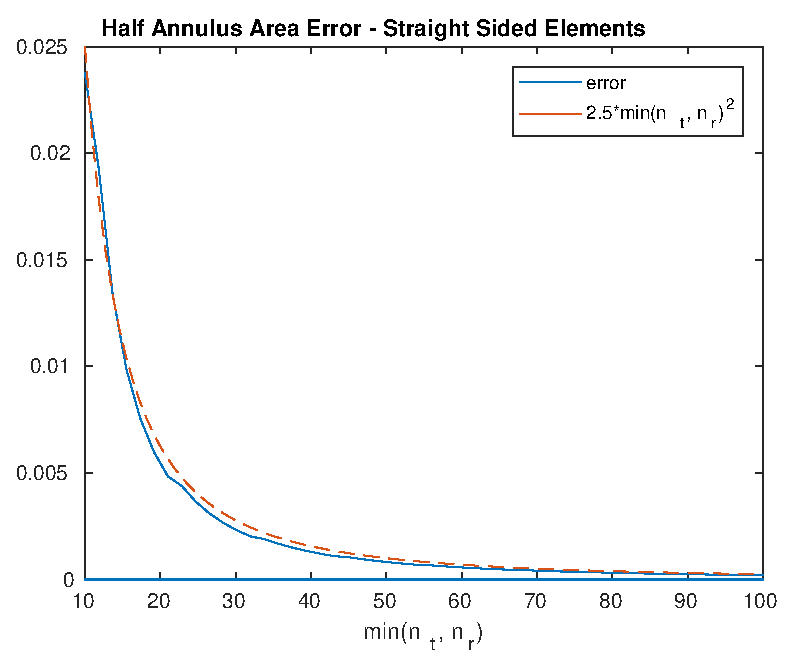
\includegraphics[scale=0.7]{media/5-3-error.eps}
  
  \caption{Error on area for curvilinear elements.}
  \label{fig:ref2}
\end{figure}

\noindent As before, we notice that we get steadily decreasing error until we achieve around $11-12$ digits of accuracy, after which roundoff errors steadily increase the error in the computation of the derivative. 

\section{Mapping with Curvi-Linear Quadrilaterals}

\subsection{Gordon-Hall Mapping}
\noindent To remedy to convergence issue with straight-sided quadrilaterals, we look into mapping the reference domain to a curvilinear domain. As a case study, we look at the half annulus as described in the homework PDF. 
% Our half annulus can be defined as the region where $\frac{1}{2}\leq r\leq 1$ and $0\leq\pi\leq 1$, plotted below:

% \begin{figure}[H]
%   \centering
%   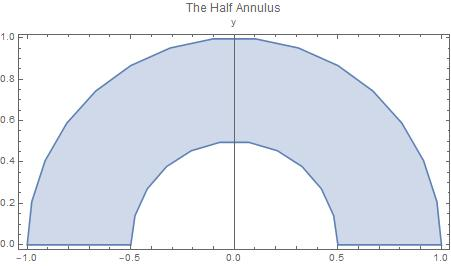
\includegraphics[width=4in]{GreensThm/HPC_HW_5_Annulus.jpg}
% \end{figure}

Green's Theorem states that for most functions P(x,y) and Q(x,y):
\begin{equation*}
\iint_{D}(\frac{\partial Q}{\partial x}-\frac{\partial P}{\partial y})dA=\oint_{C}Pdx+Qdy
\end{equation*}
D is the region being integrated over and C is the positively oriented (counterclockwise) boundary of D.\\
To compute the area of D, we integrate the function f(x,y)=1 over the region. However, we can also use Green's Theorem to compute area by choosing P and Q such that $\frac{\partial Q}{\partial x}-\frac{\partial P}{\partial y}=1$. Any P and Q that satisfy this work and the area is equal to resulting line integral $\oint_{C}Pdx+Qdy$. For this problem, it is simplest to set P=0 and Q=x. This leaves us with the formula:
\begin{equation*}
A=\oint_{C}x\space dy
\end{equation*}
The boundary of the annulus can be broken into 4 parts and parameterized as follows for $t_i\epsilon[0,1]$:\\
\begin{center}
  \begin{tabular}{|c|c|c|c|c|}
      \hline
    i & $x(t_i)$ & $y(t_i)$ & $\frac{dy_i}{dt}$ & $\vec{n}$ \\
        \hline
        1 & $\cos(\pi t)$ & $\sin(\pi t)$ & $\pi \cos(\pi t)$ & $\cos(\pi t)\hat{x}+\sin(\pi t)\hat{y}$ \\
        \hline
        2 & $\frac{t}{2}-1$ & 0 & 0 & $-\hat{y}$ \\
        \hline
        3 & $-\frac{1}{2}\cos(\pi t)$ & $\frac{1}{2}\sin(\pi t)$ & $\frac{\pi}{2} \cos(\pi t)$ & $\cos(\pi t)\hat{x}-\sin(\pi t)\hat{y}$ \\
        \hline
        4 & $\frac{t}{2}+\frac{1}{2}$ & 0 & 0 & $\hat{y}$ \\
        \hline
    \end{tabular}
\end{center}
\mbox{}\\
Curve 1 is the outer semicircle (oriented counterclockwise), curves 2 and 4 are the left and right edges along the x-axis, and curve 3 is the inner circle (oriented clockwise). When followed in order, they combine to make the boundary of the half annulus. Then our area is

  \begin{align*}
    A = \oint_{C}xdy & = \int_{0}^{1}\sum_{i=1}^{4}x_i(t)dy_i(t)dt \\
    & = \int_{0}^{1}\cos(\pi t)\cdot(\pi \cos(\pi t))+0\cdot(\frac{t}{2}-1)-\frac{1}{2}\cos(\pi t)\cdot(\frac{\pi}{2} \cos(\pi t))+0\cdot(\frac{t}{2}+\frac{1}{2})\mbox{ }dt \\
    & =\int_{0}^{1}(\pi-\frac{\pi}{4})\cdot \cos^2(\pi t)dt\\ 
    & =\frac{3\pi}{4}\left[\frac{x}{2}-\frac{\sin(2\pi x)}{4\pi}\right]_0^1 \\
    & =\frac{3\pi}{4}\cdot(\frac{1}{2}-0)=\underline{\frac{3\pi}{8}\approx1.1781}.  
  \end{align*}
\noindent If we compute the area directly using the formula for the area of a half annulus (derived from the area of a circle), we get $A=\frac{\pi}{2}\cdot(1^2-0.5^2)=\frac{\pi}{2}\cdot\frac{3}{4}=\underline{\frac{3\pi}{8}}$. For a more general domain, we will consider the Gordon-Hall mapping.

 For the outermost elements with Face $1$ on the portion of the annulus with radius $1$, we seek to find a mapping $\pi_1 : (r,s) \to (x,y)$. Let corner $1$ be denoted as $(x_s,y_s)$ and corner $2$ be denoted $x_e,y_e$. Then clearly we have 
  \begin{align*}
    \theta _s = \arctan \left(\frac{y_s}{x_s}\right), \quad \theta_e = \arctan \left(\frac{y_e}{x_e}\right),
  \end{align*}
so that a mapping $\pi_1$ from the reference domain Face $1$ to physical space Face $1$ is
  \begin{align*}
    \pi_1(r,s) = \cos \left( \theta_s + \frac{1}{2}(1 + r)(\theta_e - \theta_s) \right) \hat{\textbf{x}} + \sin \left( \theta_s + \frac{1}{2}(1 + s)(\theta_e - \theta_s) \right) \hat{\textbf{y.}}
  \end{align*}
with an analagous mapping for the elements where Face $3$ is curved and the portion of the annulus with radius $0.5$.

In order to use the mapping to compute integrals (and derivatives) we will need to compute the metric, i.e. $r_x, \, r_y, \, s_x, \, s_y$. Recall that the chain rule for a function of two variables requires that:
  \begin{align*}
    \pdiff{u(x(r,s),y(r,s))}{x} & = \pdiff{r}{x}\pdiff{u}{r} + \pdiff{s}{x} \pdiff{u}{s}, \\
    \pdiff{u(x(r,s),y(r,s))}{y} & = \pdiff{r}{y}\pdiff{u}{r} + \pdiff{s}{y} \pdiff{u}{s}.
  \end{align*}
By substituting $u = x$ and $u = y$ into the above equations, we arrive at:
  \begin{align*}
    1 & = \pdiff{x}{x} = \pdiff{r}{x}\pdiff{x}{r} + \pdiff{s}{x} \pdiff{x}{s} = r_x x_r + s_x x_s, \\
    1 & = \pdiff{y}{y}  = \pdiff{r}{y}\pdiff{y}{r} + \pdiff{s}{y} \pdiff{y}{s} = r_y y_r + s_y y_s.  
  \end{align*}
Rewriting this as a matrix system, we arrive at 

  \begin{equation}
    \begin{bmatrix}
      1 & 0 \\
      0 & 1
    \end{bmatrix}
    = 
    \begin{bmatrix}
      r_x & s_x \\
      r_y & s_y
    \end{bmatrix}
    \begin{bmatrix}
      x_r & y_r \\
      x_s & y_s
    \end{bmatrix}.
  \end{equation}
Using the explicit formula for the inverse of a matrix, we immediately solve for the metric via
  \begin{equation}
    \begin{bmatrix}
      r_x & s_x \\
      r_y & s_y
    \end{bmatrix}
    =
    \begin{bmatrix}
      x_r & y_r \\
      x_s & y_s
    \end{bmatrix}^{-1}
    = \frac{1}{x_r y_s - x_s y_r}
    \begin{bmatrix}
      y_s & -y_r \\
      -x_s & x_r
    \end{bmatrix}
    = \frac{1}{J}
    \begin{bmatrix}
      y_s & -y_r \\
      -x_s & x_r
    \end{bmatrix}.
  \end{equation}
where $J = x_r y_s - x_s y_r$. With the inversion of the metric, we may approximate the area of an element numerically via

  \begin{align*}
    V =  \int_\Omega 1 \, dV = \int_{-1}^1 \int_{-1}^1 J \, dx\,dy \approx \sum_{i = 0}^n \sum_{j=0}^n w_j w_i J(x_j, y_i).
  \end{align*}
  Below is a plot of the area approximation of the annulus with a subdivision of 4 elements (2 in the radial direction, and 2 in the angular direction).
  \begin{figure}[H]
    \centering
    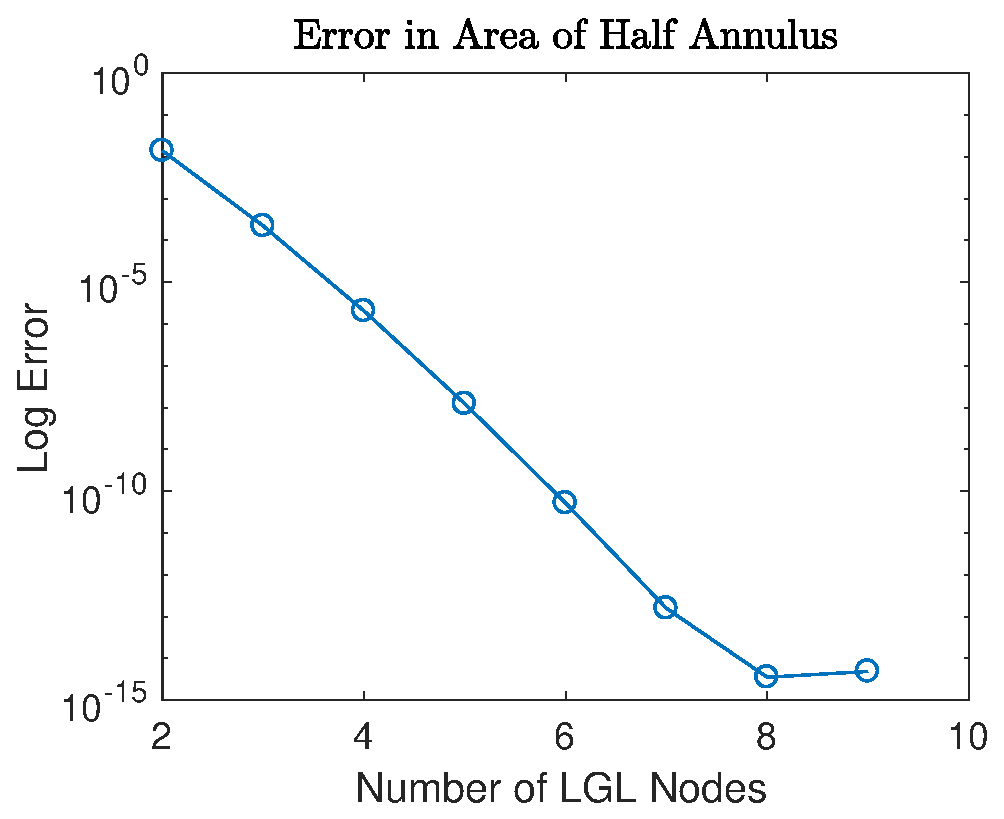
\includegraphics[scale=0.7]{media/GHannulus.eps}
    \caption{Plot of Error with Increasing $N$}
    \label{fig:annulus_plot}
  \end{figure}
\noindent We note that taking into account the curvilinearity of the outer elements yields especially fast convergence of the area to the true value of $\frac{3\pi}{8}$.

\subsection{Line Integrals}
We now consider finding the area of an element via line integrals (instead of the previously direct volume integral). To that end, consider the vector field $F(x,y) = (x/2, y/2)$. Then $\nabla \cdot F(x,y) = 1$ and by the divergence theorem:

  \begin{align*}
    V =  \int_\Omega 1 \, dV = \int_\Omega \nabla \cdot F(x,y) \, dV = \int_{\partial \Omega} \nabla F(x,y) \cdot \hat{\textbf{n}} \, dl = \int_{\partial \Omega} \left( \frac{x}{2}n_1 + \frac{y}{2}n_2 \right)\, dl,
  \end{align*}
where $\hat{\textbf{n}} = (n_1,n_2)$. If we consider the reference square, side 1 corresponds to $s = 1$ and $r \in [-1,1]$. The tangent to the curve along this face is clearly $(x_r,y_r)$ so that the normal is
  \begin{align*}
    (-y_r, \, x_r) = J (s_x, \, s_y) \implies \hat{\boldsymbol{n_1}} = \frac{(s_x, \, s_y)}{\sqrt{s_x^2 + s_y^2}}.
  \end{align*}
A similar calculation for the other 3 faces will yield the following set of normals (where the subscript indicates which face it belongs to):

  \begin{align*}
    \hat{\boldsymbol{n_1}} = \frac{(s_x, \, s_y)}{\sqrt{s_x^2 + s_y^2}}, & \quad
    \hat{\boldsymbol{n_2}} = -\frac{(r_x, \, r_y)}{\sqrt{r_x^2 + r_y^2}}, \\
    \hat{\boldsymbol{n_3}} = -\frac{(s_x, \, s_y)}{\sqrt{s_x^2 + s_y^2}}, & \quad
    \hat{\boldsymbol{n_4}} = \frac{(r_x, \, r_y)}{\sqrt{s_x^2 + s_y^2}}. \\
  \end{align*}
Using these, we repeat the previous area calculation of the annulus via line integrals around the boundary of each element. Below is a plot of the error with increasing number of quadrature nodes (given 4 total elements - 2 in the radial direction and 2 in the angular direction):

\begin{figure}[H]
  \centering
  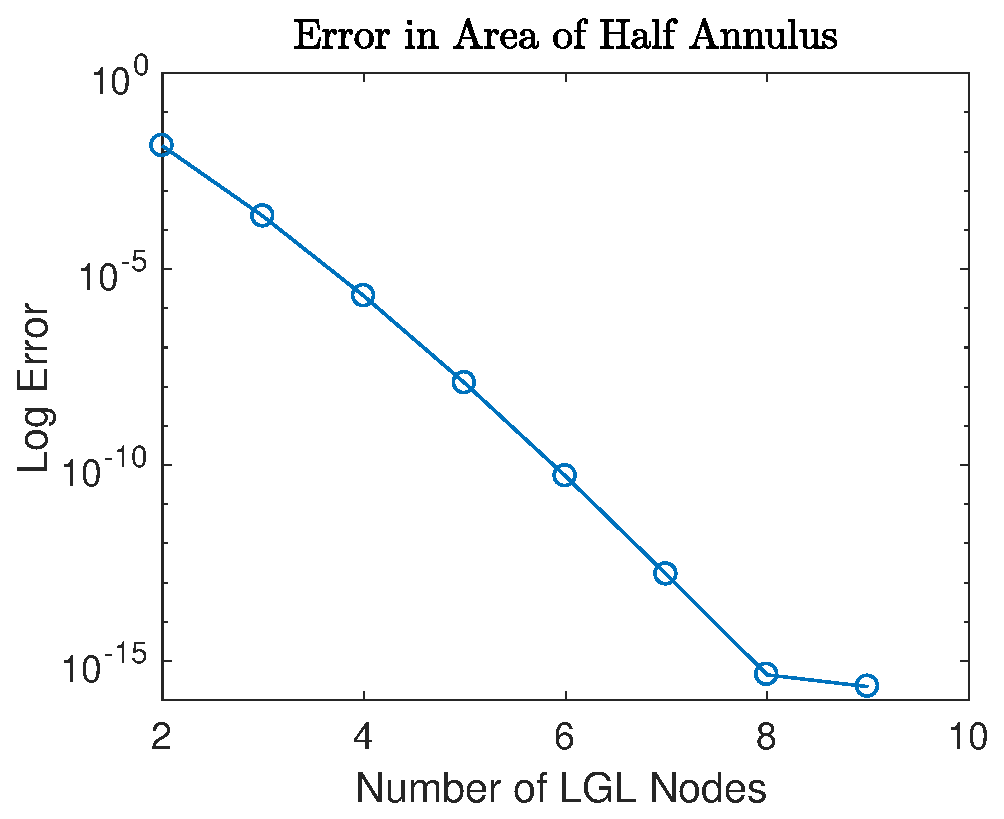
\includegraphics[scale=0.7]{media/annulus_line.eps}
  \caption{Plot of Error with Increasing $N$}
  \label{fig:line_plot}
\end{figure}
\noindent We note that we begin with 2 digits of accuracy and with as little as 8 quadrature nodes per side we get an error of the order of machine precision.

\subsection{$L_2$ Projection}
We next consider the approximation via Legendre polynomials in $2$ dimensions. That is, we wish to find the coefficients of an element wise approximation
  \begin{align*}
    u^h(x(r,s),y(r,s)) = \sum_{k = 0}^q \sum_{l = 0}^q \hat{u}_{k,l}^h P_k(r)P_l(s).
  \end{align*}
As done on a previous homework, we determine the coefficients by multiplying and integrating against Legendre polynomials:
  \begin{align*}
    \int_{-1}^1 \int_{-1}^1 u^h(x(r,s),y(r,s)) P_m(r)P_n(s) J \, dr \, ds  & = \int_{-1}^1 \int_{-1}^1 \sum_{k = 0}^q \sum_{l = 0}^q \hat{u}_{k,l}^h P_k(r)P_l(s)P_m(r)P_n(s) J \, dr \, ds, \\
    & = \sum_{k = 0}^q \sum_{l = 0}^q \hat{u}_{k,l}^h \int_{-1}^1 \int_{-1}^1 P_k(r)P_l(s)P_m(r)P_n(s) J \, dr \, ds,
  \end{align*}
  which we may rewrite as the matrix equation
    \begin{align*}
      M \hat{u} = b,
    \end{align*}
where 
  \begin{align*}
    M_{m,n} = \int_{-1}^1 \int_{-1}^1 P_k(r)P_l(s)P_m(r)P_n(s) J \, dr \, ds,
  \end{align*}
and
  \begin{align*}
    b_n = \int_{-1}^1 \int_{-1}^1 u^h(x(r,s),y(r,s)) P_m(r)P_n(s) J \, dr \, ds,
  \end{align*}
and where $n = i + j(q+1)$. An implementation for the function $f(x,y) = \cos \left(2\pi\right) x \sin \left(2\pi y\right)$ was done and the error plot is below:
\begin{figure}[H]
  \centering
  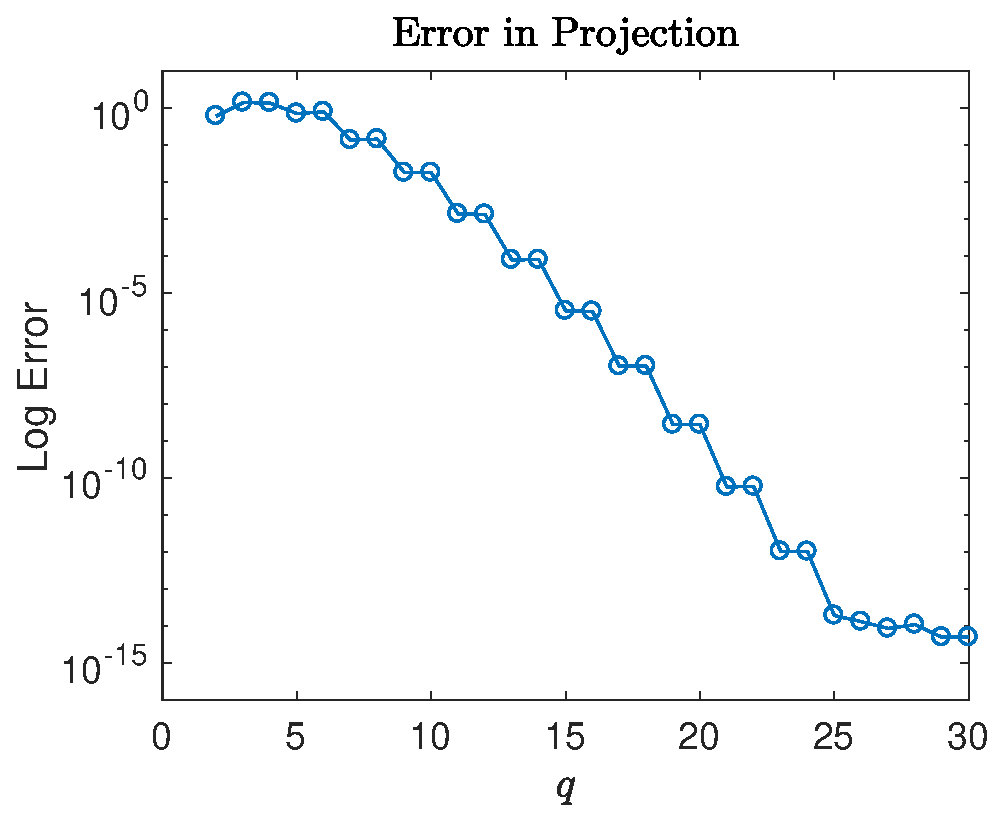
\includegraphics[scale=0.7]{media/coeff_error.eps}
  \caption{Plot of Error with Increasing $q$}
  \label{fig:coeff_plot}
\end{figure}
\noindent We note that we begin to get digits of accuracy starting at around $q = 10$ and that the error decreases via pairs of doubles, likely due to the fact that the initial data is an even function.
\subsection{Differentiation}
Finally, we'll wish to compute $u_x$ and $u_y$. Note that via the chain rule:
  \begin{align*}
    u_x^h = \pdiff{r}{x}\pdiff{u^h}{r}  + \pdiff{s}{x}\pdiff{u^h}{s} = r_x u_r^h + s_x u_s^h,
  \end{align*}
and for $y$,
  \begin{align*}
    u_y^h = \pdiff{r}{y}\pdiff{u^h}{r}  + \pdiff{s}{y}\pdiff{u^h}{s} = r_y u_r^h + s_y u_s^h.
  \end{align*}
Taking derivatives of our expansion we have 
  \begin{align*}
    \pdiff{u^h}{r} = \pdiff{}{r}\left[ \sum_{k = 0}^q \sum_{l = 0}^q \hat{u}_{k,l}^h P_k(r)P_l(s) \right] = \sum_{k = 0}^q \sum_{l = 0}^q \hat{u}_{k,l}^h P_k'(r)P_l(s),
  \end{align*}
and similarly for $s$. Subsitution into our chain rule yields:

  \begin{align*}
    u_x^h & = r_x \left[ \sum_{k = 0}^q \sum_{l = 0}^q \hat{u}_{k,l}^h P_k'(r)P_l(s) \right] + s_x \left[ \sum_{k = 0}^q \sum_{l = 0}^q \hat{u}_{k,l}^h P_k(r)P_l'(s) \right], \\
    & = \sum_{k = 0}^q \sum_{l = 0}^q \hat{u}_{k,l}^h \left( r_x P_k'(r)P_l(s) + s_x P_k(r)P_l'(s) \right).
  \end{align*}
which we may evaluate directly to approximate $u_x$. Similarly for $y$:
  \begin{align*}
    u_y^h & = r_y \left[ \sum_{k = 0}^q \sum_{l = 0}^q \hat{u}_{k,l}^h P_k'(r)P_l(s) \right] + s_y \left[ \sum_{k = 0}^q \sum_{l = 0}^q \hat{u}_{k,l}^h P_k(r)P_l'(s) \right], \\
    & = \sum_{k = 0}^q \sum_{l = 0}^q \hat{u}_{k,l}^h \left( r_y P_k'(r)P_l(s) + s_y P_k(r)P_l'(s) \right).
  \end{align*}
Below is a plot of the error in computing the derivatives of $u(x,y) = \cos \left(2\pi\right) x \sin \left(2\pi y\right)$ on a single element.
\begin{figure}[H]
  \centering
  \begin{minipage}{.6\textwidth}
    \centering
    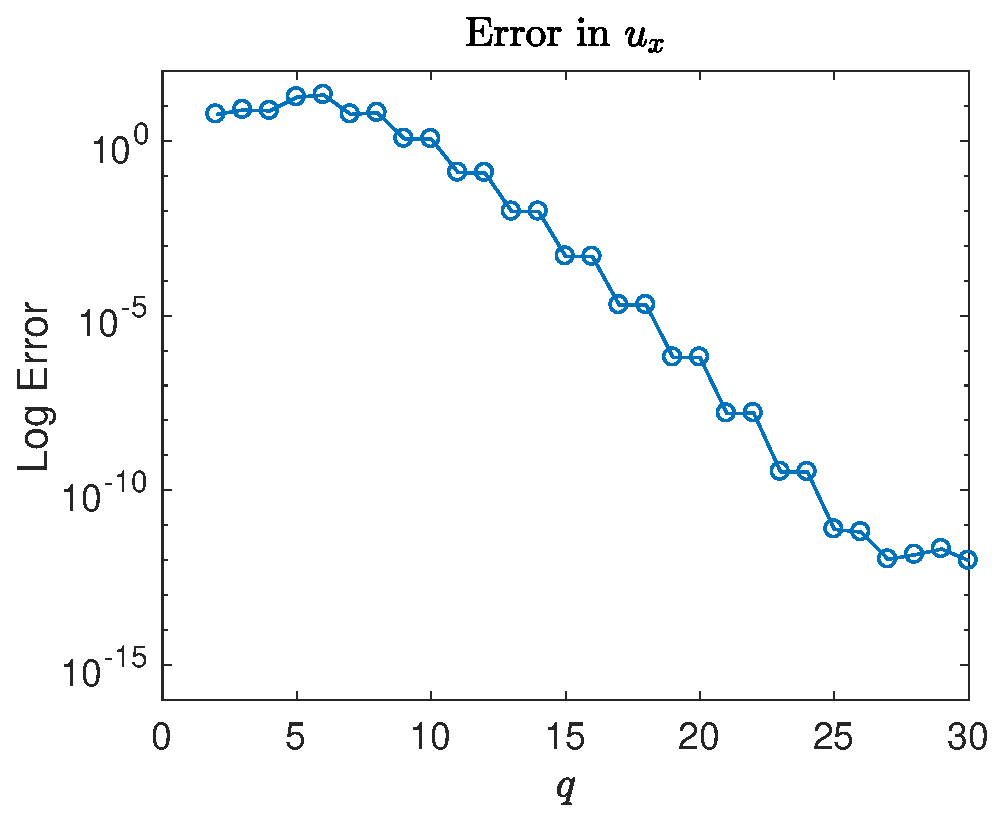
\includegraphics[width=\linewidth]{media/derivative_x_error.eps}
    \caption{Error in $u_x$}
    \label{fig:beta0}
  \end{minipage}%
  \begin{minipage}{.6\textwidth}
    \centering
    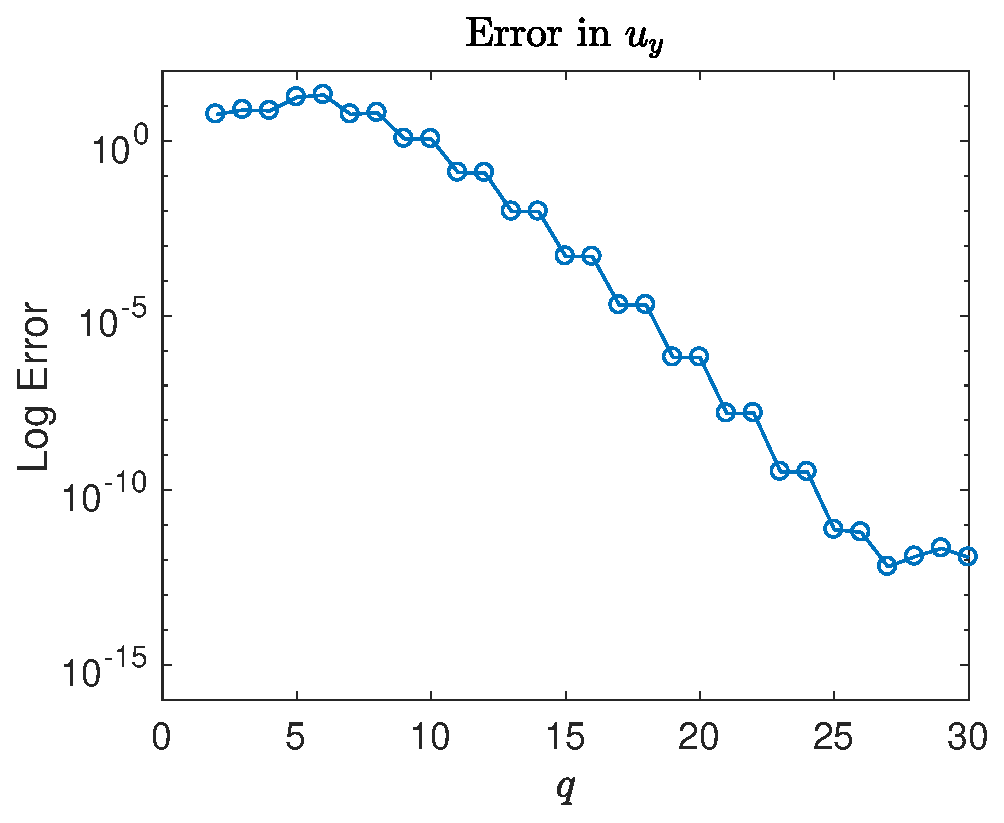
\includegraphics[width=\linewidth]{media/derivative_y_error.eps}
    \caption{Error in $u_y$}
    \label{fig:beta1}
  \end{minipage}%
\end{figure}
\noindent Similar to the error in projecting initial data, we note that we begin to get digits of accuracy at around $q = 10$ and accuracy increases overall as $q$ increases.






\end{document}


